\subsection{Aire Guru}

Aire Guru utiliza los datos de calidad del aire proporcionados por el ayuntamiento de Malaga en su portal de datos abiertos.\footnote{\url{https://datosabiertos.malaga.eu/}}
\begin{figure}[h]
    \centering
   \subfigure[Pagina principal]
    {\includegraphics[width=5.5cm  ]{OpenDataPortal}}
    \hfill
    \subfigure [Categoria medio ambiente]
       { 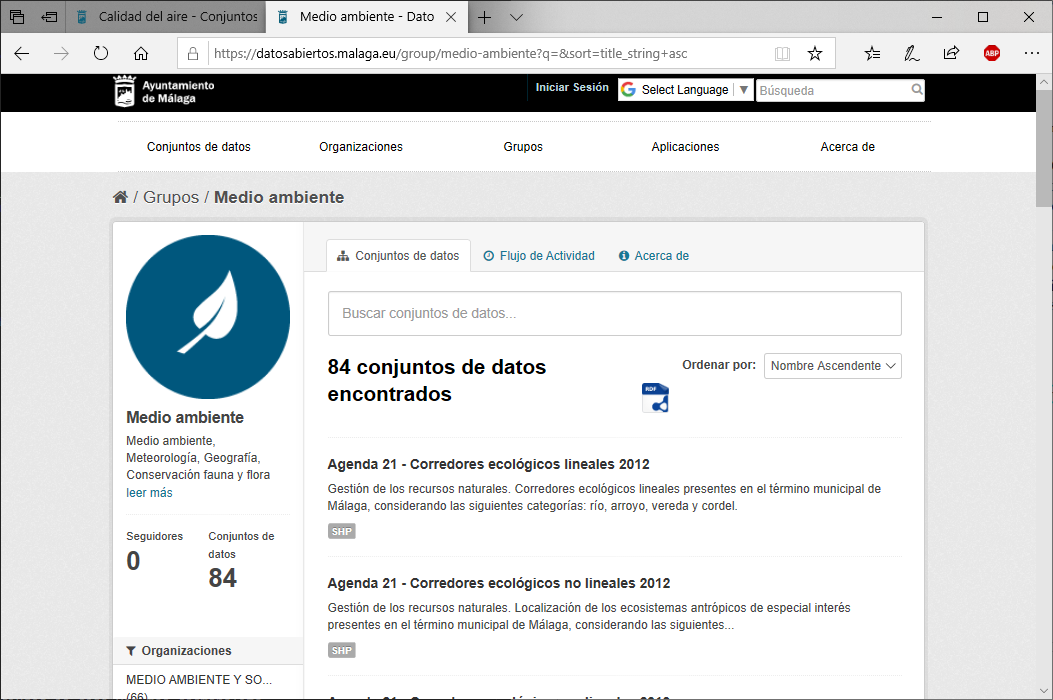
\includegraphics[width=5.5cm]{openDataPortalEnviromentCategory}}
  
  \caption{Open Data Portal Malaga}
    \end{figure}
Este portal de datos ofrece una oferta de categorias representados por iconos, por lo que es necesario saber en que categoria se clasifica el conjunto
de datos, una vez que se accede a la categoria, tenemos una barra buscadora que nos permite insertar las palabras claves para buscar el conjunto de datos
deseado.\\

Los datos extraidos estan en formato GeoJSON, este formato proporciona un objeto JSON con subdocumentos anidados, cada uno de estos
subdocumentos contiene un conjunto de datos en forma clave valor. 
En la siguiente figura podemos ver el principio del documento descargado el 09 de Junio del 2019 
\footnote{\url{https://datosabiertos.malaga.eu/recursos/ambiente/calidadaire/calidadaire.json}}\\
\newpage
\begin{figure}[h]
    \centering
   \subfigure[Primer subdocumento]{ \centering 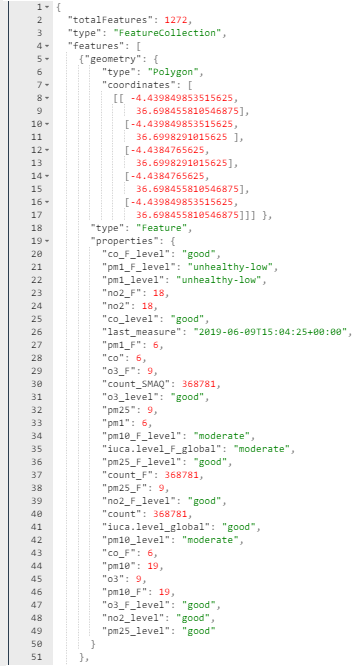
\includegraphics[width=4.75cm]{geoJsonAirQualityData1}}
   \hfill
   \subfigure[Segundo subdocumento]{ \centering 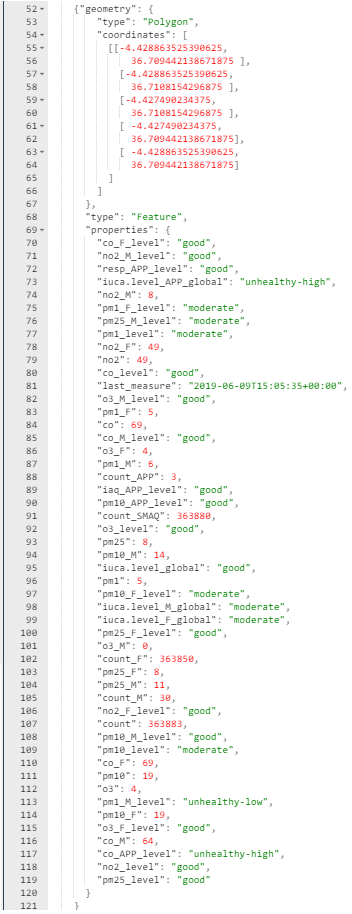
\includegraphics[width=4.75cm]{geoJsonAirQualityData2}}
    \caption{Air quality Document [09/06/2019].Open Data Portal Malaga}
    \end{figure}
    
En este extracto podemos ver los primeros dos subdocumentos. Cada subdocumento contiene las coordenadas de la estacion medidora de la calidad
del aire, la fecha y hora cuando se registro la medida y a continuacion los valores de las mediciones. 
En la figura siguiente podemos encontrar la descripcion proporcionada por el portal de datos abiertos.
\begin{figure}[ht]
    \centering
    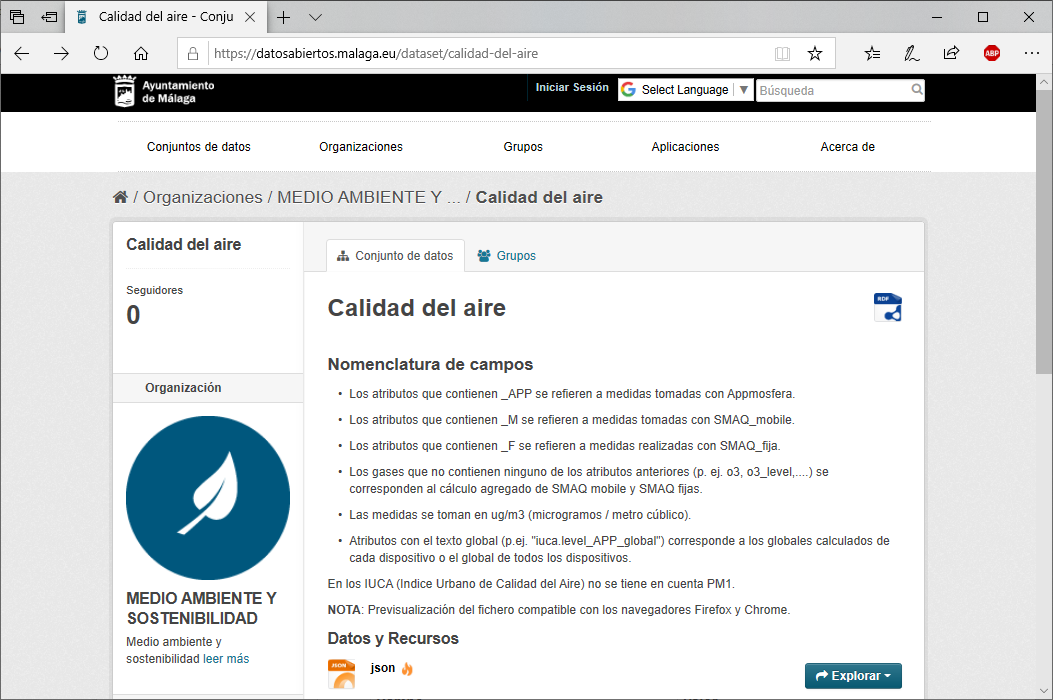
\includegraphics[width=8cm]{geoJsonAirQualityDataDescription}
    \caption{Air quality data description [09/06/2019].Open Data Portal Malaga}
\end{figure}

Para una descripcion mas en detalle de las medidas, tenemos que recurrir a un recurso externo, en este caso nos pusimos en contacto directamente con
la empresa que instala las estaciones de medida UrbanClouds \footnote{\url{https://urbanclouds.city/es/}} y proporciona los datos al ayuntamiento de Malaga.

Una pregunta simple seria saber a que nivel de polucion estamos rodeados en las coordenadas en la que nos encontramos. Con la informacion en 
crudo obtenida desde el portal, nos es una tarea imposible, pero si ardua si no contamos con un sistema que procese los datos.

Aire Guru se ocupa de representar el EAQI (European Air Quality Index) general calculado sobre un mapa. Este es un formato mas legible para los usuarios.
Este indice mustra un indicador con cinco niveles: "Insalubre" "Malo" "Pobre" "Aceptable" y "Bueno" y especifica un rango de colores desde el rojo hasta el celeste.

\begin{figure}[ht]
    \centering
    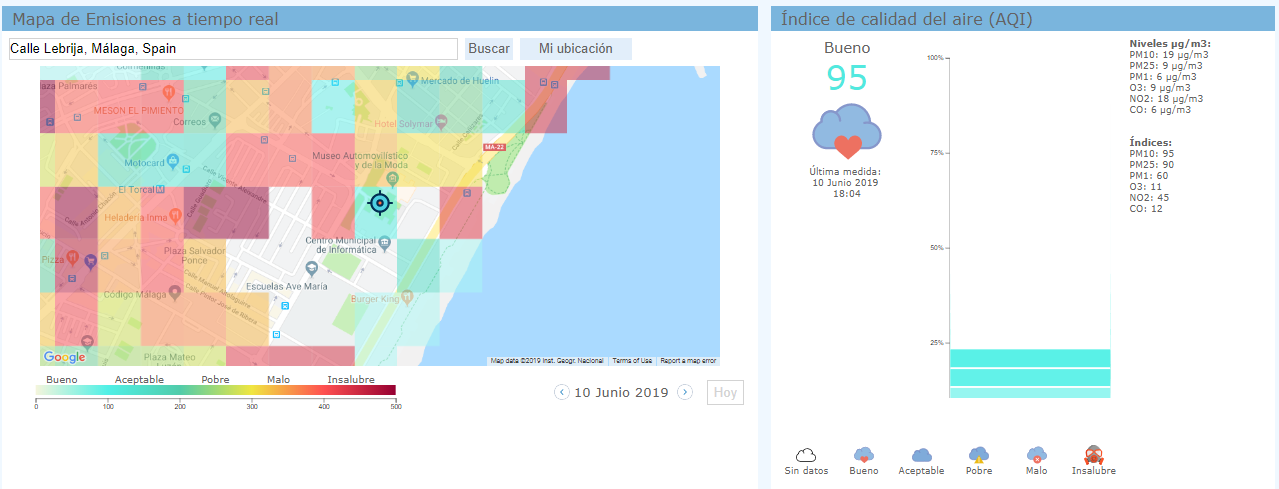
\includegraphics[width=12cm]{mapAireGuru}
    \caption{Aire Guru. Landing page. Top section}
\end{figure}
Nuestra plataforma introduce ademas una iconografica para ayudar al usuario a tener una idea directa de la situacion, ya que son mas 
explicativos que los colores. En caso de peligro, queda bien representado con el color rojo, pero en el caso del azul o verde, en nuestra cultura, no
tenemos definido un estado para estos colores.
\begin{figure}[ht]
    \centering
    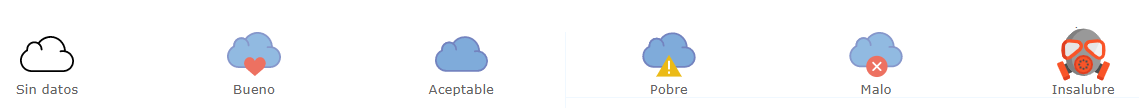
\includegraphics[width=12cm]{EAQUI_Icons}
    \caption{Iconografica Aire Guru}
\end{figure}
\newpage

La herramienta Aire guru presenta la informacion en el idioma nativo de la ciudad y se utiliza un lenguaje sencillo y directo.
Ademas se utiliza el mismo estilo, colores e iconografia en todo el diseno para que el usuario se familierize rapidamente y pueda
prestar atencion al significado de los datos en vez de perderse en el diseno e intentar encontrar su significado.

Para garantizar el alcance a la mayoria de la poblacion, Aire Guru esta disponible en las direcciones webs https://www.aire.guru y https://www.airquality.guru.
Usa SSL que garantiza la encriptacion de los datos atraves de la red, ademas, cada vez mas navegadores intentan proteger a los usuarios y
solo muestran paginas que utilizar un metodo seguro. 

Aire Guru se comprende de distintas secciones disponibles para todos los usuarios. En la zona superior, podemos ver el mapa que mediante la seleccion de un punto, nos
mostrara informacion detallada de este punto. A continuacion, cuenta con una seccion que filtrara la informacion acorde a las preferencias del usuario
y para concluir, muestra el historial de los contaminantes desde 2018.
Ademas, para usuarios identificados, mostrara directamente la informacion de su localizacion y mostrara al usuario su historial personal
con la polucion a la que ha estado rodeado.

Como vemos, todos los usuarios pueden ver la informacion basica sin necesidad de aportar ningun dato o identificarse, sin la necesidad de 
realizar ninguna descarga o instalacion y hoy en dia, casi todo el mundo esta familiarizado con la navegacion web.

El workflow de las distintas secciones de Aire Guru esta detalladamente estudiada. Como vemos en la Figura X. Aire Guru. Landing page. Top section, el punto de partida es la localizacion que nos interesa,
a continuacion se muestra la informacion general de este punto, el AQI general, despues el AQI de cada uno de los contaminantes que componen el 
AQI general y por ultimo los valores numericos de cada uno de los contaminantes. Como vemos vamos de menos a mas detalle.

Por ultimo, Aire Guru cuenta con un glosario, donde explica que significa el indice de calidad del aire y como se calcula. 
Ademas, cuenta con multiples enlaces externos donde el usuario puede obtener mas informacion.


